% Particle CLEM in PeleC: operators, anchored energy coupling and AMR
% Build: latexmk -pdf main.tex
\documentclass[aspectratio=169,10pt]{beamer}

\usepackage[T1]{fontenc}
\usepackage{amsmath,amssymb,bm}
\usepackage{booktabs}
\usepackage{tikz}
\usetikzlibrary{arrows.meta,positioning,calc,fit}

% ---- minimal look -----------------------------------------------------------
\usefonttheme{professionalfonts}
\setbeamertemplate{navigation symbols}{}
\setbeamertemplate{itemize items}{\textendash}
\setbeamertemplate{footline}{\hfill\scriptsize\color{gray}\insertframenumber\hspace{2mm}\vspace{2mm}}
\definecolor{accent}{RGB}{31,94,166}
\setbeamercolor{frametitle}{fg=black}
\setbeamercolor{title}{fg=black}
\setbeamercolor{structure}{fg=accent}
\setbeamerfont{frametitle}{size=\large,series=\bfseries}
\setbeamertemplate{frametitle}{\vspace{2mm}\insertframetitle\par\vspace{-1mm}{\color{gray!40}\rule{\textwidth}{0.4pt}}}

\tikzset{
  op/.style={draw, rounded corners=2pt, minimum height=7mm, minimum width=13mm, align=center, font=\small},
  les/.style={op, fill=gray!10},
  flow/.style={-{Stealth[length=2mm]}, thick},
  dot/.style={circle, fill=black, inner sep=0pt, minimum size=1.6pt},
  cdot/.style={circle, draw=red!70!black, inner sep=0pt, minimum size=2.4pt},
}

% ---- operators --------------------------------------------------------------
\newcommand{\F}{\mathcal{F}}          % forward coupling
\renewcommand{\L}{\mathcal{L}}        % line processes
\newcommand{\Sig}{\Sigma^{\omega}}    % splice
\newcommand{\R}{\mathcal{R}}          % regrid
\newcommand{\B}{\mathcal{B}}          % backward coupling
\newcommand{\A}{\mathcal{A}}          % energy anchor
\renewcommand{\H}{\mathcal{H}}        % halo
\newcommand{\M}{\mathcal{M}}          % mass reflux
\newcommand{\D}{\mathcal{D}}          % average down
\newcommand{\C}{\mathcal{C}}          % refine: children
\newcommand{\K}{\mathcal{K}}          % coarsen
\newcommand{\Pl}{\mathcal{P}}         % a line
\newcommand{\filt}[1]{[#1]_c}

\title{Particle CLEM in PeleC}
\author{Fernando Illacanchi Guerra, PUCP}
\date{15.10.2026}

\begin{document}

% =============================================================================
\begin{frame}[plain]
  \titlepage
\end{frame}

% =============================================================================
\begin{frame}{LEM and LES}
\small
\begin{columns}[T]
\begin{column}{0.48\textwidth}
\textbf{LES} (PeleC, MOL--RK2), $Y_k$ not solved here
\[
U_c = \big[\rho,\ \rho\mathbf{u},\ \rho E \big],\quad E = e + \tfrac12|\mathbf{u}|^2
\]
\textbf{Line} $\Pl_c$ AMReX particles in \emph{every} cell of \emph{every} level, ordered by \texttt{lem\_index} (head $=0$)
\[
p \in \Pl_c:\ \ \big(m_p,\, v_p,\, \rho_p,\, T_p,\, e_p,\, P_p,\, Y_{k,p}\big),\ \ \rho_p = \frac{m_p}{v_p}
\]
\end{column}
\begin{column}{0.48\textwidth}
\textbf{Conserved filter}
\[
\filt{\rho\phi} = \frac{1}{V_c}\sum_{p\in\Pl_c} m_p\,\phi_p ,\qquad \phi \in \{1,\ Y_k,\ e\}
\]

\textbf{Mass-weighted filter}
\[
\filt{\phi} = \frac{1}{m_c}\sum_{p\in\Pl_c} m_p\,\phi_p ,\qquad \phi \in \{1,\ Y_k,\ e\}
\]


\textbf{Ownership}
\begin{itemize}
  \item LES: $\rho$, $\rho\mathbf{u}$, $\rho E$
  \item lines: $Y_k$ and $e$(needed for Reaction) (transport, diffusion, reaction)
\end{itemize}
\textbf{Face mass flux} kept per level, RK2 average
\[
\ F = \rho^{*}u^{*}A,\ \ \mu_f = \Delta t\,|\dot m_f|
\]
\end{column}
\end{columns}
\end{frame}

% =============================================================================
\begin{frame}{PeleC AMR time stepping}
\begin{columns}[c]
\begin{column}{0.5\textwidth}
\centering
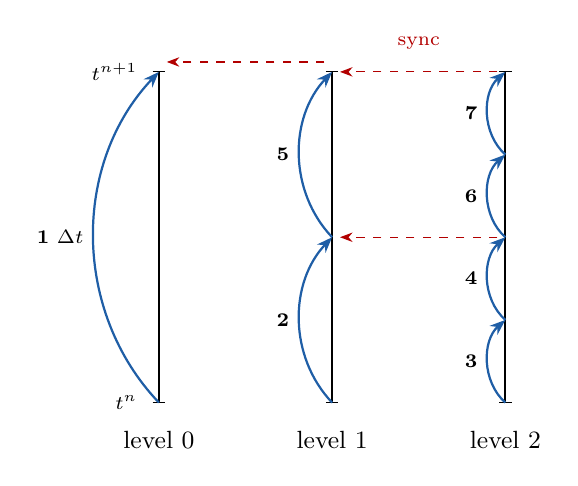
\begin{tikzpicture}[yscale=1.05]
  % three time axes of equal length, one per level, from t^n to t^{n+1}
  \foreach \l/\x in {0/0, 1/2.2, 2/4.4} {
    \draw[thick] (\x,0) -- (\x,4);
    \node[font=\small] at (\x,-0.45) {level \l};
  }
  \foreach \x in {0,2.2,4.4} {\draw (\x-0.08,0) -- (\x+0.08,0); \draw (\x-0.08,4) -- (\x+0.08,4);}
  \node[font=\scriptsize, anchor=east] at (-0.15,0) {$t^n$};
  \node[font=\scriptsize, anchor=east] at (-0.15,4) {$t^{n+1}$};
  % level 0: one step of Delta t
  \draw[flow, accent] (0,0) to[bend left=45] node[left,font=\scriptsize,black]{\textbf{1}\ $\Delta t$} (0,4);
  % level 1: two steps of Delta t / 2
  \draw[flow, accent] (2.2,0) to[bend left=45] node[left,font=\scriptsize,black]{\textbf{2}} (2.2,2);
  \draw[flow, accent] (2.2,2) to[bend left=45] node[left,font=\scriptsize,black]{\textbf{5}} (2.2,4);
  % level 2: four steps of Delta t / 4
  \draw[flow, accent] (4.4,0) to[bend left=50] node[left,font=\scriptsize,black]{\textbf{3}} (4.4,1);
  \draw[flow, accent] (4.4,1) to[bend left=50] node[left,font=\scriptsize,black]{\textbf{4}} (4.4,2);
  \draw[flow, accent] (4.4,2) to[bend left=50] node[left,font=\scriptsize,black]{\textbf{6}} (4.4,3);
  \draw[flow, accent] (4.4,3) to[bend left=50] node[left,font=\scriptsize,black]{\textbf{7}} (4.4,4);
  % syncs: fine onto coarse when both are at the same time
  \draw[-{Stealth[length=1.6mm]}, dashed, red!70!black] (4.3,2) -- (2.3,2);
  \draw[-{Stealth[length=1.6mm]}, dashed, red!70!black] (4.3,4) -- (2.3,4);
  \draw[-{Stealth[length=1.6mm]}, dashed, red!70!black] (2.1,4.12) -- (0.1,4.12);
  \node[font=\scriptsize, red!70!black] at (3.3,4.35) {sync};
\end{tikzpicture}
\end{column}
\begin{column}{0.48\textwidth}
\small
\textbf{Subcycling in time}, refinement ratio $r = 2$
\[
\Delta t_{\ell} = \frac{\Delta t_0}{r^{\ell}}
\]
\begin{itemize}
  \item Reflux is the syncronization of the fluxes at the coarse/fine interface. Not trivial in particle advection.
  \item Need to make decision of what information can be lost,
\end{itemize}

\end{column}
\end{columns}
\end{frame}

% =============================================================================
\begin{frame}{One step as a composition of operators}
\centering\small
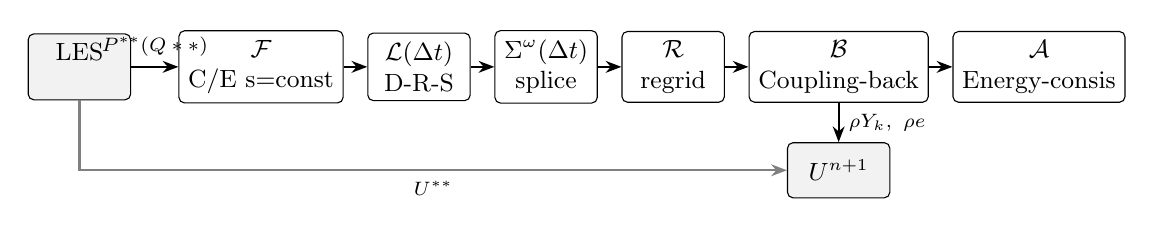
\begin{tikzpicture}[node distance=4mm and 3mm, every node/.append style={font=\footnotesize}]
  \node[les] (rk) {LES\\ };
  \node[op, right=6mm of rk] (F) {$\F$\\ C/E s=const };
  \node[op, right=of F] (L) {$\L(\Delta t)$\\ D-R-S};
  \node[op, right=of L] (S) {$\Sig(\Delta t)$\\ splice};
  \node[op, right=of S] (R) {$\R$\\ regrid};
  \node[op, right=of R] (B) {$\B$\\ Coupling-back};
  \node[op, right=of B] (A) {$\A$\\ Energy-consis};
  \draw[flow] (rk) -- node[above,font=\scriptsize]{$P^{**}(Q**)$} (F);
  \draw[flow] (F) -- (L); \draw[flow] (L) -- (S); \draw[flow] (S) -- (R);
  \draw[flow] (R) -- (B); \draw[flow] (B) -- (A);
  \node[les, below=5mm of B] (U) {$U^{n+1}$};
  \draw[flow] (B) -- node[right,font=\scriptsize]{$\rho Y_k,\ \rho e$} (U);
  \draw[flow, gray] (rk.south) |- node[below,pos=0.75,font=\scriptsize,black]{$U^{**}$} (U.west);
\end{tikzpicture}

\vspace{1mm}
\begin{minipage}{0.92\textwidth}
\textbf{Level step} ($\ell$, its own $\Delta t_\ell$, in place of \texttt{react\_state})
\[
\Pl^{\,n+1}_{\ell} = \A\circ\B\circ\R\circ\Sig(\Delta t_\ell)\circ\L(\Delta t_\ell)\circ\F\ \big[\Pl^{\,n}_{\ell}\big]
\]
\textbf{Coarse/fine sync} (\texttt{post\_timestep} of $\ell$) and \textbf{AMR regrid}
\[
\Pl_\ell \leftarrow \D_{\ell+1\to\ell}\circ\B_{\delta}\circ\R\big|_{\partial}\circ\M\ \big[\Pl_\ell\big],
\qquad
\Pl \leftarrow \D\circ\K\circ\C\ \big[\Pl\big]
\]
Particle reflux, regrid, couple-back, and average down. $\delta m$ is conserved(not necessarily $\delta \phi$)
\end{minipage}
\end{frame}

% =============================================================================
\begin{frame}{Line operations}
\footnotesize
\begin{columns}[T]
\begin{column}{0.49\textwidth}
\textbf{$\F$ forward coupling} (isentropic, frozen $Y$), $\Pi = P^{**}/P_p$

\textbf{$\L$ diffusion} (mass coordinate $dm = \rho A\,dx$, isobaric, periodic line)
\[
\frac{DY_k}{Dt} = RHS(Y_k)
\]

\[
\frac{DT}{Dt} = RHS(T) + \frac{1}{\rho c_v}\sum_k h_k\,RHS(Y_k)
\]
explicit integration
\end{column}
\begin{column}{0.49\textwidth}
\textbf{$\Sig$ splice}, outflux faces $N^+_c$, influx faces $N^-_c$
\[
\sigma_f = \mathrm{Cut}_{\mu_f}\big(\text{head of }\Pl_c\big),\quad f \in \mathcal{O}^{\omega}(N^+_c)
\]

$\mathcal{O}^{+}$: $|\mu|$ descending,\ $\mathcal{O}^{-}$: ascending,\ alternating: $\omega_n = (-1)^{n+1}$\\
{Strang composition $\mathcal{O}^+ ...\mathcal{O}^- $}\\[1mm]


\vspace{2mm}
\textbf{$\R$ regrid} to $n_{\mathrm{lem}}$ equal-mass elements. Conservation of $m$, $v$, $\sum m Y_k$, $\sum m e$
\end{column}
\end{columns}
\end{frame}


% =============================================================================
\begin{frame}{Particle advection: splicing}
\small
Advection of a square-shaped scalar field along the diagonal (2D, single level)
\begin{center}
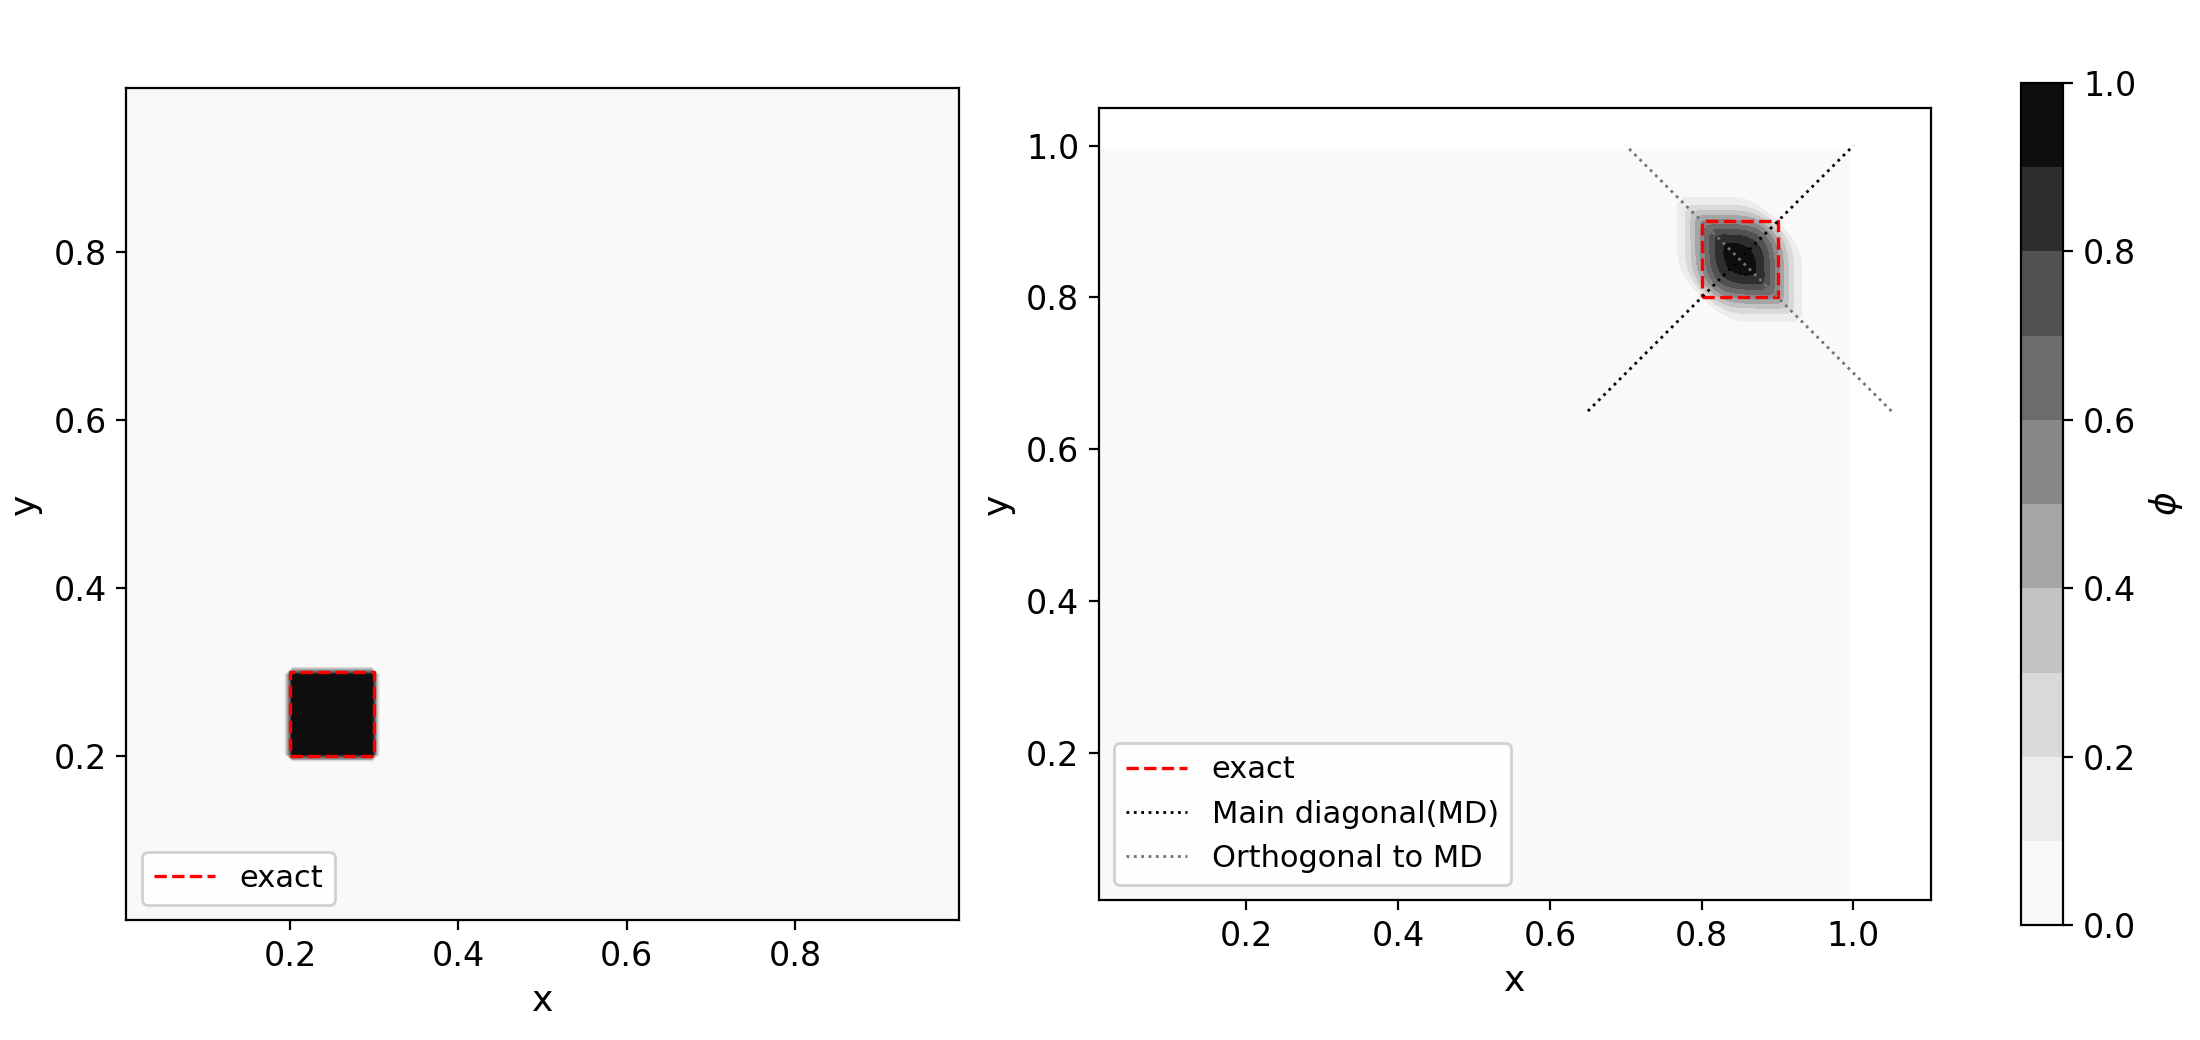
\includegraphics[height=2.6cm]{figs/splicing_field.png}\hspace{3mm}
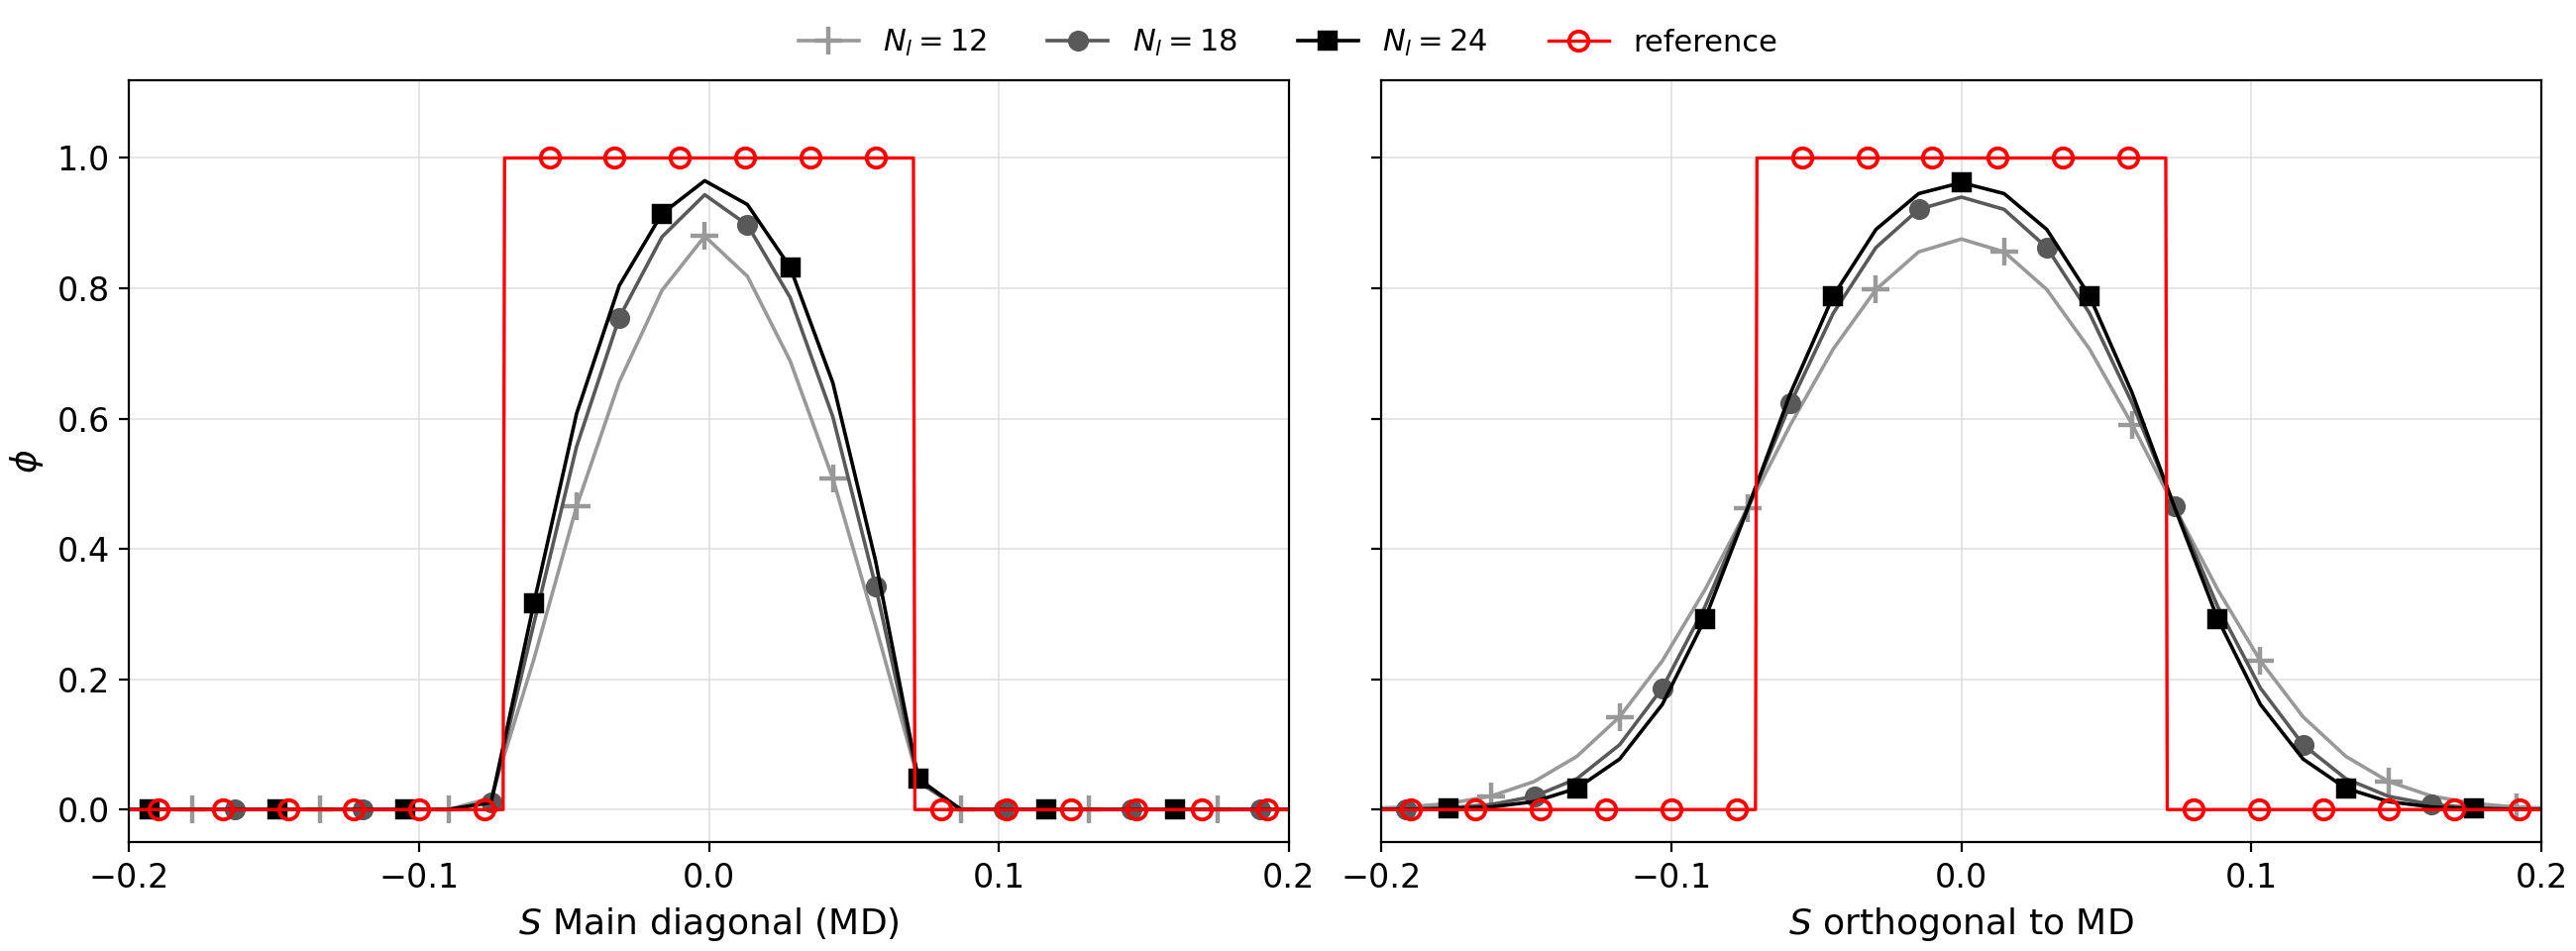
\includegraphics[height=2.6cm]{figs/splicing_profiles.png}
\end{center}
\vspace{-2mm}
{\scriptsize scalar along the main diagonal (left) and orthogonal to it (right) for $N_l = 12,\ 18,\ 24$ particles per cell}
\begin{itemize}
  \item a three-dimensional transport represented by one-dimensional lines; the total scalar is conserved by the particle method
  \item the numerical diffusion is orthogonal to the mean flow direction, and decreases with the number of particles
\end{itemize}
\end{frame}

% =============================================================================
\begin{frame}{Coupling back $\B$: LEM lines $\to$ LES}
\small
\textbf{Species}: conserved variation of a filtered scalar
\[
\Delta[\rho Y_k] = \filt{\rho Y_k}^{\mathrm{post}} - \filt{\rho Y_k}^{\mathrm{pre}},\qquad
\widetilde{\rho Y_k} = (\rho Y_k)^{n} + \Delta[\rho Y_k]
\]
mass species projection
\[
(\rho Y_k)^{n+1} = \rho^{**}\,\frac{\widetilde{\rho Y_k}}{\sum_j \widetilde{\rho Y_j}}
\qquad\Longrightarrow\qquad \sum_k Y_k^{n+1} = 1
\]

\vspace{2mm}
\textbf{Total energy}: the LES accounts for the subgrid effect
\[
(\rho E)^{n+1} = (\rho E)^{**} + \Delta[\rho e]_{\L},\qquad
\Delta[\rho e]_{\L} = \filt{\rho e}\big|_{\text{after }\L} - \filt{\rho e}\big|_{\text{before }\L}
\]

\end{frame}

% =============================================================================
\begin{frame}{Internal energy consistency $\A$: LES $\to$ lines}
\small
\begin{columns}[T]
\begin{column}{0.54\textwidth}

\[
\delta e_c = e^{n+1}_c - \bar e_c,\qquad \bar e_c = \frac{\sum_p m_p e_p}{\sum_p m_p}
\]
$\delta e_c$ internal energy difference between LES and LEM(relevant in AMR)
\[
e_p \leftarrow e_p + \delta e_c
\]
Shift from particle internal values to make internal energy consistency.

\end{column}
\begin{column}{0.44\textwidth}
\centering
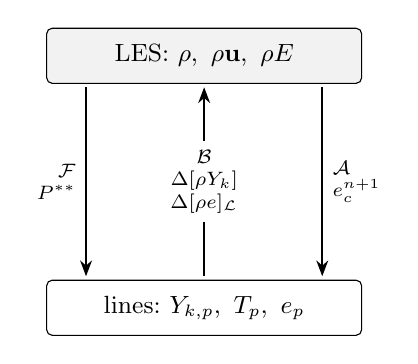
\begin{tikzpicture}
  \node[les, minimum width=40mm] (les) at (0,0) {LES:\ $\rho,\ \rho\mathbf{u},\ \rho E$};
  \node[op, minimum width=40mm] (lin) at (0,-3.2) {lines:\ $Y_{k,p},\ T_p,\ e_p$};
  \draw[flow] (-1.5,-0.4) -- (-1.5,-2.8) node[midway,left,font=\scriptsize,align=right]{$\F$\\ $P^{**}$};
  \draw[flow] (0,-2.8) -- (0,-0.4) node[midway,fill=white,font=\scriptsize,align=center]{$\B$\\ $\Delta[\rho Y_k]$\\ $\Delta[\rho e]_{\L}$};
  \draw[flow] (1.5,-0.4) -- (1.5,-2.8) node[midway,right,font=\scriptsize,align=left]{$\A$\\ $e^{n+1}_c$};
\end{tikzpicture}

\vspace{3mm}
at $t^{n+1}$ LES and lines agree in mass, energy and composition; the LES stays conservative
\end{column}
\end{columns}
\end{frame}

% =============================================================================
\begin{frame}[fragile]{Species and their enthalpy flux effect}
\small
\textbf{Problem}: the species are frozen during $RK_2$, energy and species diffusion at LES 
are set zero $\mathbf{J}_k$ (consistency between species diffusion and energy transport) 

\[
\partial_t(\rho Y_k) + \underbrace{\nabla\!\cdot(\rho Y_k\mathbf{u}) + \nabla\!\cdot\mathbf{J}_k}_{=\,0\ \text{(frozen)}} = 0,\qquad
\partial_t(\rho E) + \dots = \dots - \nabla\!\cdot\Big(\textstyle\sum_k h_k\mathbf{J}_k\Big)
\]


\vspace{3mm}
\textbf{Fix}: when the lines own the species, both are dropped on the same face
\[
\mathbf{J}_k = 0 \quad\text{and}\quad \sum_k h_k\mathbf{J}_k = 0\qquad\text{in the LES}
\]


\end{frame}

% =============================================================================
\begin{frame}{Premixed flame}
\small
Lean H$_2$--air premixed flame, $\phi = 0.4$, 300\,K, 1\,atm: 128 cells $\times$ 12 particles against a 512-cell reference
\begin{center}
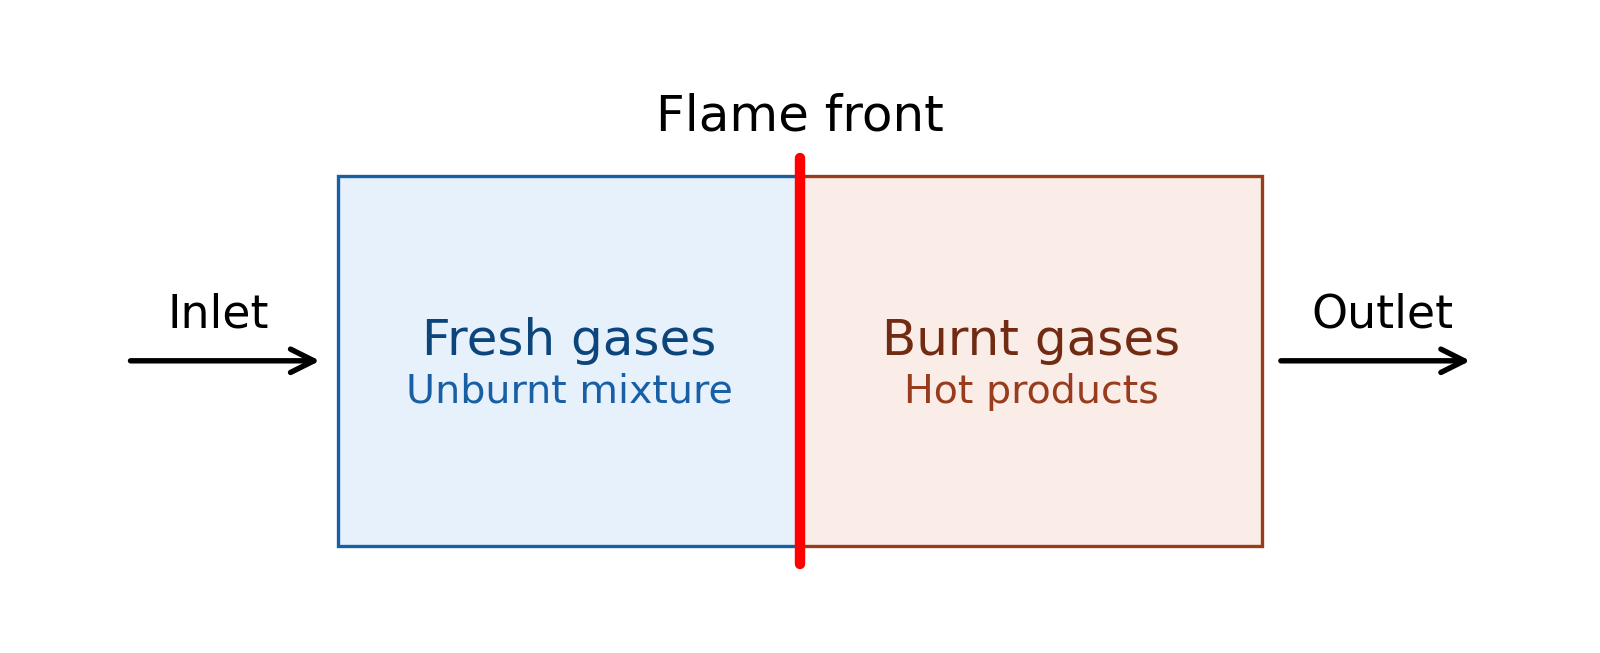
\includegraphics[height=2.6cm]{figs/pmf_schematic.png}\\[1mm]
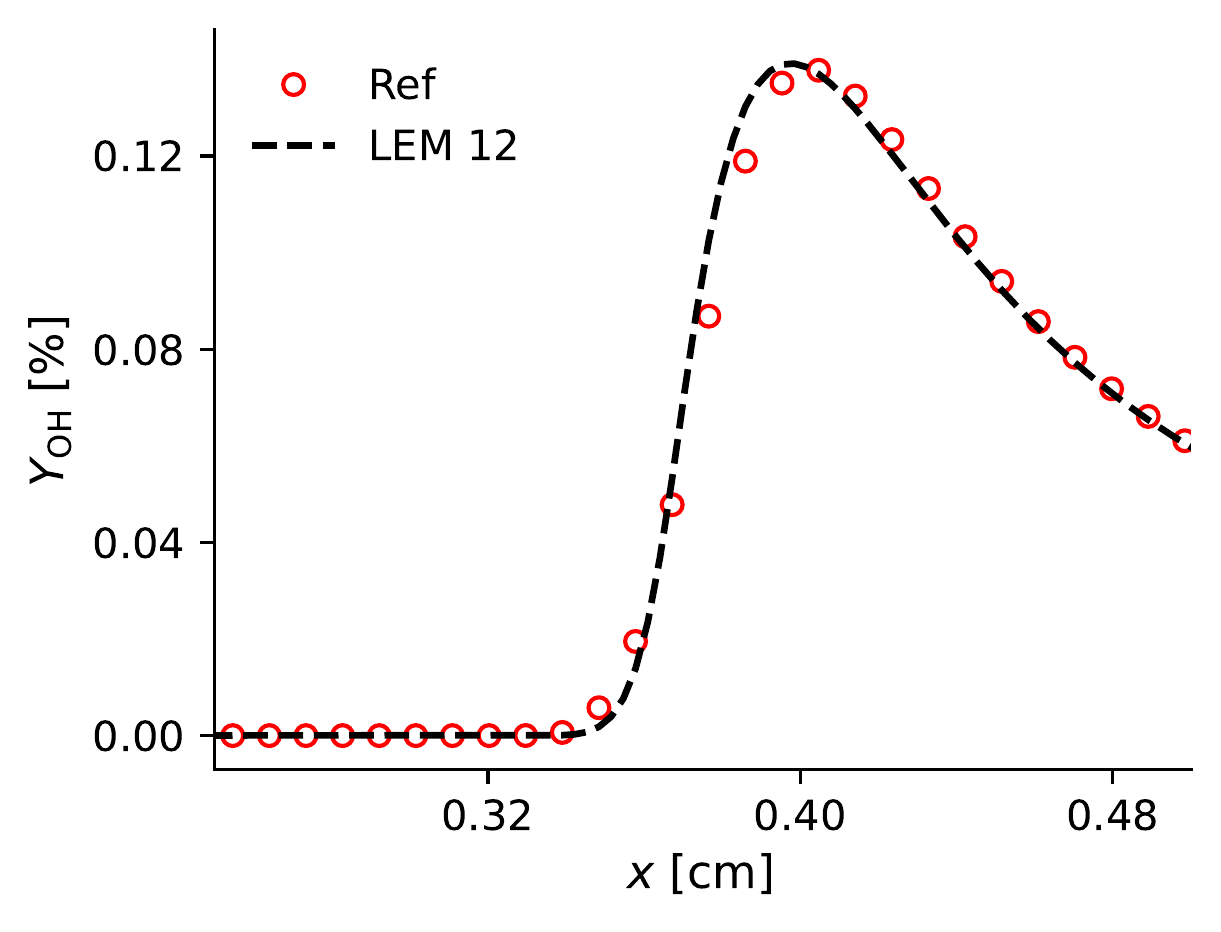
\includegraphics[height=3.4cm]{figs/pmf_OH.png}\hspace{6mm}
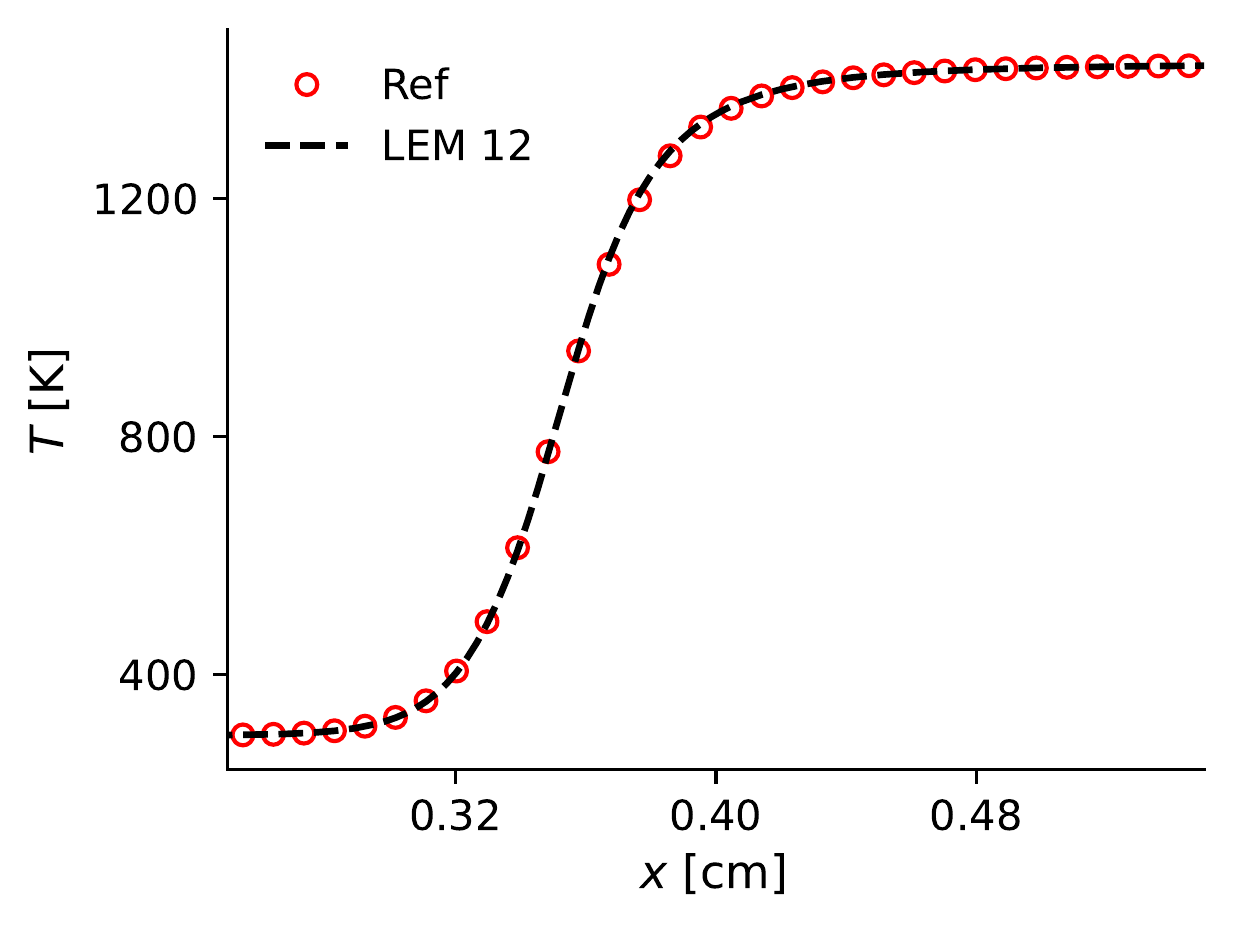
\includegraphics[height=3.4cm]{figs/pmf_T.png}
\end{center}
\vspace{-2mm}
{\scriptsize OH mass fraction (left) and temperature (right); the heat release is carried by the particle internal energy, the small shift in the species curve comes from the splicing}
\end{frame}

% =============================================================================
\begin{frame}{AMR: lines on every level}
\begin{columns}[T]
\begin{column}{0.42\textwidth}
\centering
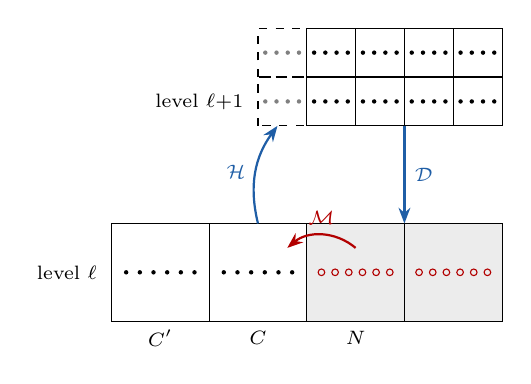
\begin{tikzpicture}[scale=0.62]
  % coarse level: 4 cells; cells 3 and 4 covered by the fine level
  \foreach \i in {0,1,2,3} {
    \draw (2*\i,0) rectangle ++(2,2);
    \foreach \k in {0,...,5} \node[dot] at (2*\i+0.3+0.28*\k,1) {};
  }
  \fill[gray!15] (4,0) rectangle (8,2);
  \foreach \i in {2,3} \foreach \k in {0,...,5} \node[cdot] at (2*\i+0.3+0.28*\k,1) {};
  \foreach \i in {0,1,2,3} \draw (2*\i,0) rectangle ++(2,2);
  \node[font=\scriptsize, anchor=east] at (-0.1,1) {level $\ell$};
  \node[font=\scriptsize] at (1,-0.35) {$C'$};
  \node[font=\scriptsize] at (3,-0.35) {$C$};
  \node[font=\scriptsize] at (5,-0.35) {$N$};
  % fine level above the covered cells
  \foreach \i in {0,...,3} \foreach \j in {0,1} {
    \draw (4+\i,4+\j) rectangle ++(1,1);
    \foreach \k in {0,...,3} \node[dot] at (4.15+\i+0.23*\k,4.5+\j) {};
  }
  \foreach \j in {0,1} {
    \draw[dashed] (3,4+\j) rectangle ++(1,1);
    \foreach \k in {0,...,3} \node[dot, fill=gray] at (3.15+0.23*\k,4.5+\j) {};
  }
  \node[font=\scriptsize, anchor=east] at (2.9,4.5) {level $\ell{+}1$};
  % operators
  \draw[flow, accent] (3,2) to[bend left=25] node[left,font=\scriptsize]{$\H$} (3.4,4);
  \draw[flow, accent] (6,4) -- node[right,font=\scriptsize]{$\D$} (6,2);
  \draw[flow, red!70!black] (5,1.5) to[bend right=40] node[above,font=\scriptsize]{$\M$} (3.6,1.5);
\end{tikzpicture}

\vspace{2mm}
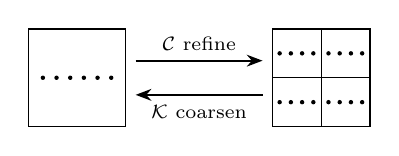
\begin{tikzpicture}[scale=0.62]
  \draw (0,0) rectangle (2,2); \foreach \k in {0,...,5} \node[dot] at (0.3+0.28*\k,1) {};
  \foreach \i in {0,1} \foreach \j in {0,1} {
    \draw (5+\i,\j) rectangle ++(1,1);
    \foreach \k in {0,...,3} \node[dot] at (5.15+\i+0.23*\k,0.5+\j) {};
  }
  \draw[flow] (2.2,1.35) -- node[above,font=\scriptsize]{$\C$ refine} (4.8,1.35);
  \draw[flow] (4.8,0.65) -- node[below,font=\scriptsize]{$\K$ coarsen} (2.2,0.65);
\end{tikzpicture}
\end{column}
\begin{column}{0.56\textwidth}
\footnotesize
\textbf{$\H$ halo}: clone of the coarse line, same state, $\big(m_k, v_k\big)/r^{d}$\\[1mm]
\textbf{$\M$ particle mass reflux}, per interface face
\[
\delta\mu_f = \sum_s \mu^{s}_{f,\mathrm{fine}} - \mu_{f,\mathrm{coarse}}
\]
Reflux follows the splicing rule. Then regriding $\R$ on $C$, and 
species coupling following coupling-back.

\textbf{$\D$ average down}, element $k$ over the $r^d$ children
\[
m_k = \sum_c m_{c,k},\quad v_k = \sum_c v_{c,k},\quad \psi_k = \frac{\sum_c m_{c,k}\,\psi_{c,k}}{m_k}
\]
$\psi \in \{e,\ Y_k\}$, then $T_k = T(\rho_k, e_k, Y_k)$\\[1mm]
\textbf{$\C$ refine}: children are clones with $m/r^d$; LES filled piecewise constant\\
\textbf{$\K$ coarsen}: fine lines dropped; the parent already holds $\D$
\end{column}
\end{columns}
\end{frame}




% =============================================================================
\begin{frame}{Particle topology on the AMR hierarchy}
\small
\begin{columns}[T]
\begin{column}{0.49\textwidth}
\centering
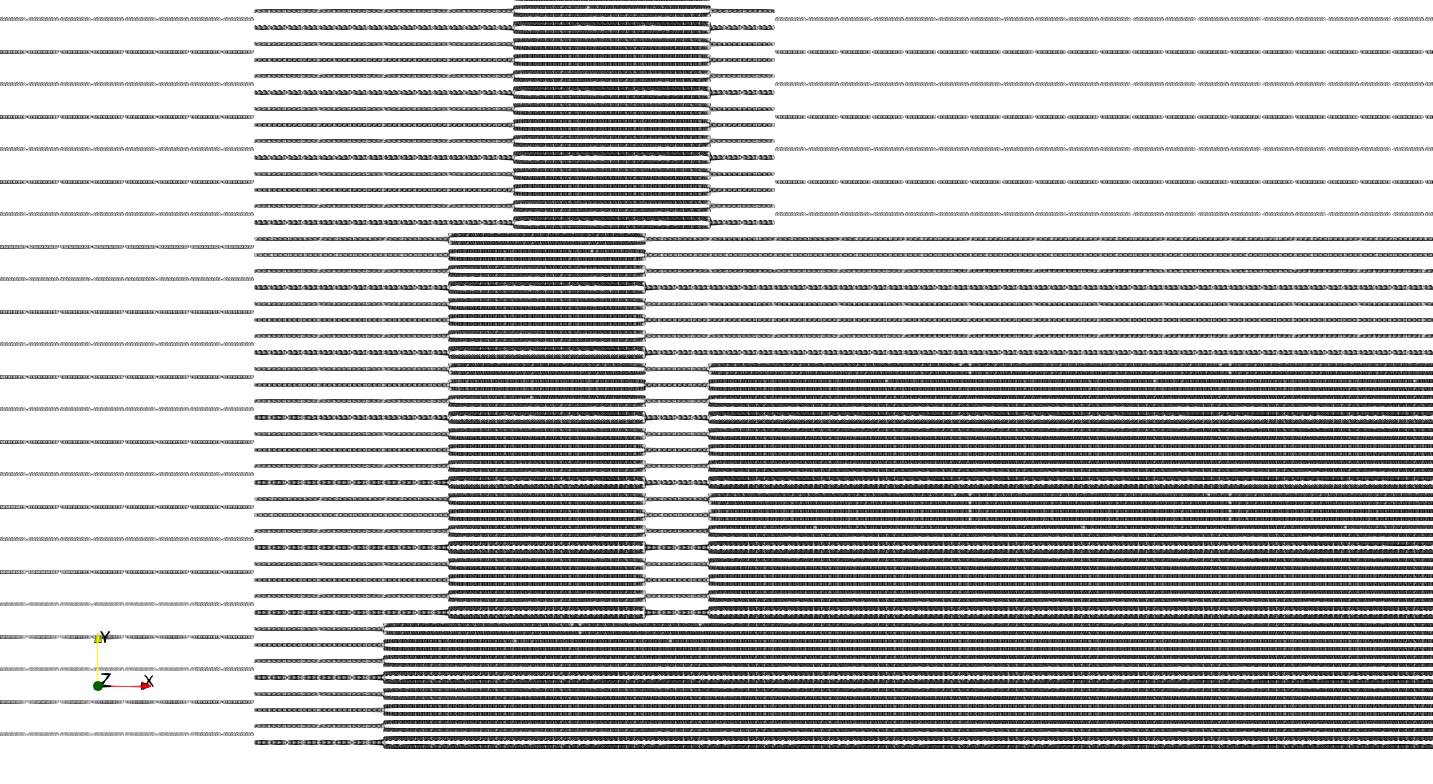
\includegraphics[width=\textwidth]{figs/particle_topology.png}\\[1mm]
{\scriptsize one LEM line per cell on every level: the lines follow the block structure and are denser on the finer levels}
\end{column}
\begin{column}{0.49\textwidth}
\centering
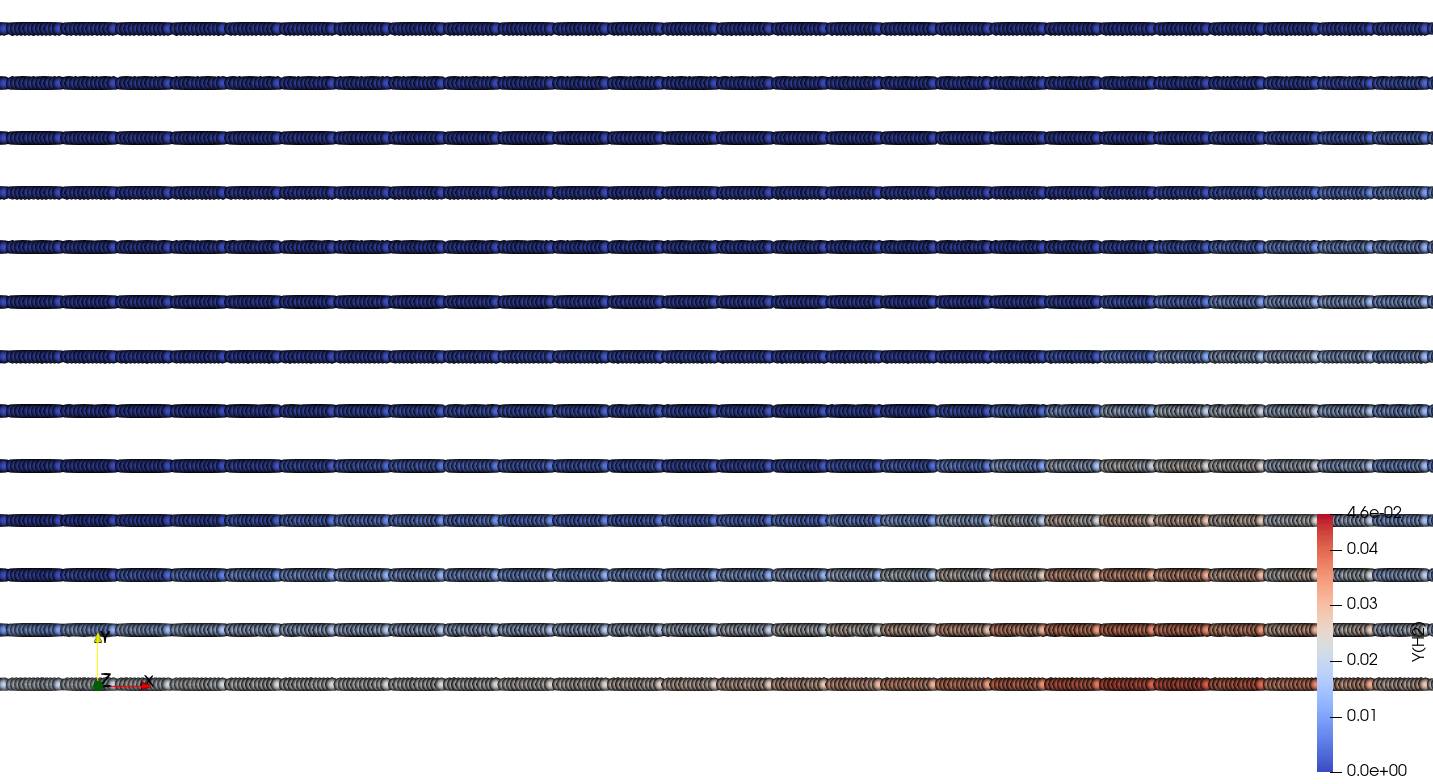
\includegraphics[width=\textwidth]{figs/h2_particle_topology.png}\\[1mm]
{\scriptsize elements coloured by $Y_{\mathrm{H_2}}$: the sub-grid structure carried along each line}
\end{column}
\end{columns}
\end{frame}

% =============================================================================
\begin{frame}{H$_2$ jet in supersonic crossflow (2D), $t = 0.25$\,ms}
\centering
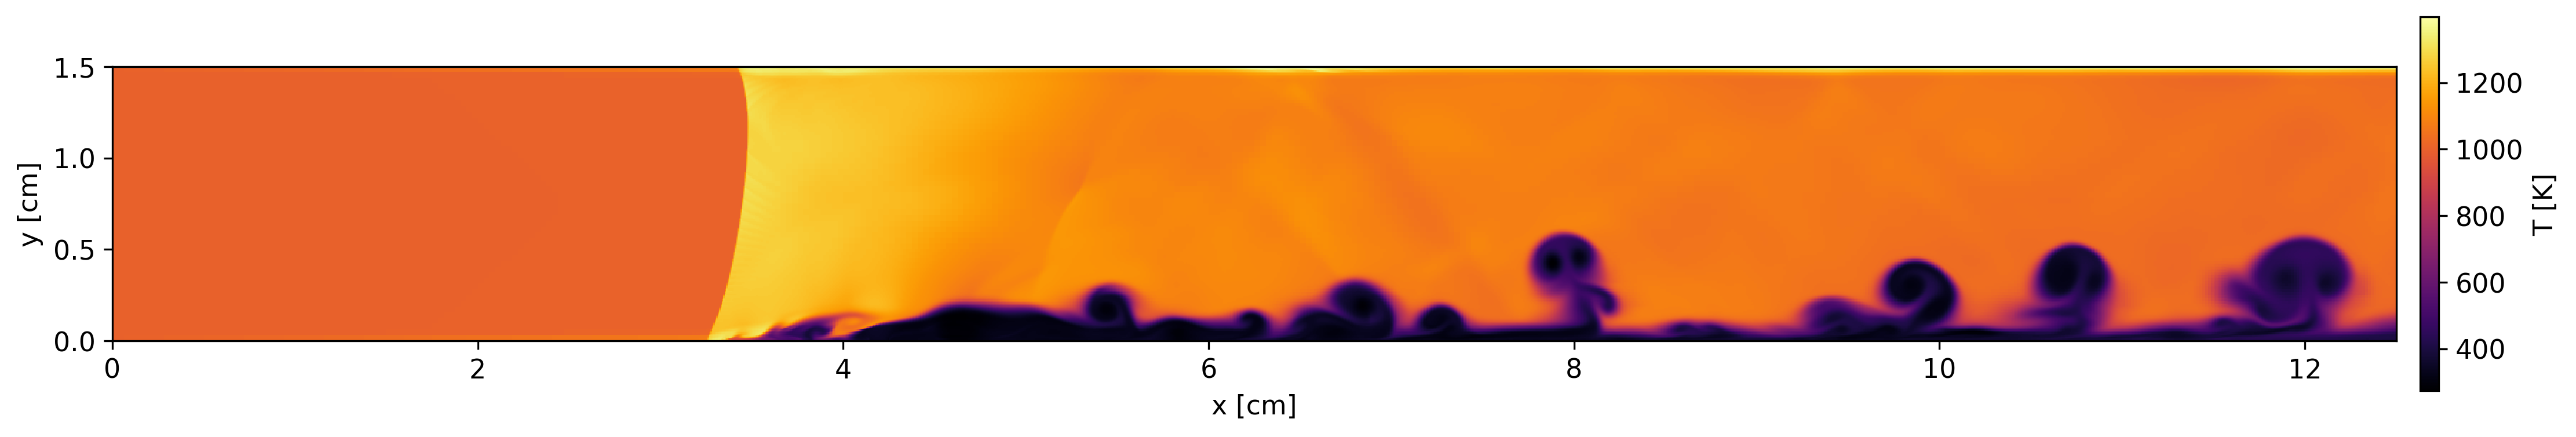
\includegraphics[width=0.95\textwidth]{figs/T_t0.25ms.png}\\[2mm]
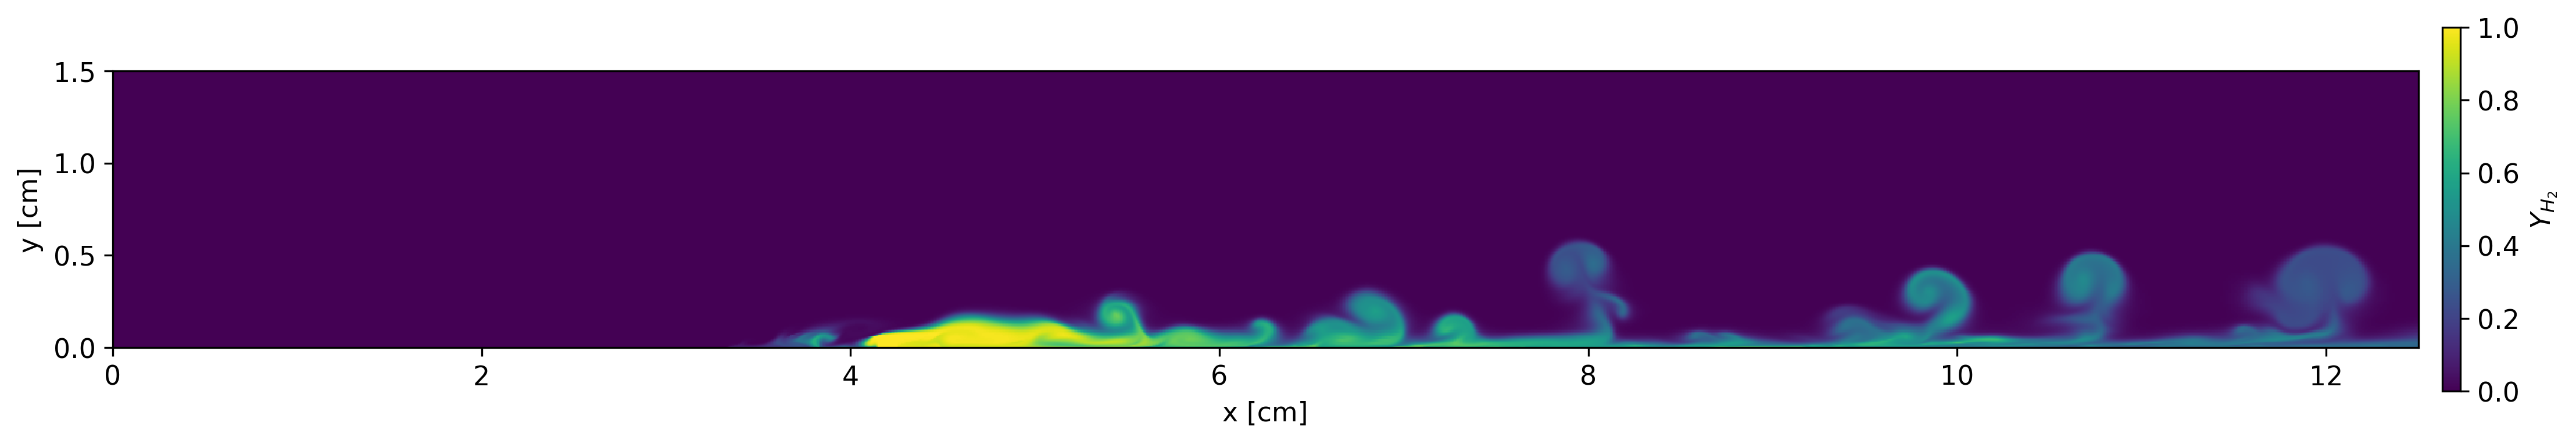
\includegraphics[width=0.95\textwidth]{figs/YH2_t0.25ms.png}\\[1mm]
{\scriptsize temperature (top) and H$_2$ mass fraction (bottom)}
\end{frame}

\end{document}
